\documentclass[../../main]{subfiles}

\begin{document}
\chapter{数ベクトル空間}
\label{chapter:numerical_vector_space}

\begin{lead}
  準備中.
\end{lead}

\section{直交射影}

本節では,あるベクトルを他のベクトルの線型結合で近似する手法を説明する.
特に断りのない限り,\cref{chapter:numerical_vector_space}において\(\innerp{\holder}{\holder}\)は\(\numset{C}^n\)の標準内積を意味する.
また
\[
  \vnorm{\vect{x}} = \sqrt{\innerp{\vect{x}}{\vect{x}}}
  = \sqrt{\abs{x_1}^2+\dots+\abs{x_n}^2}
  \quad\text{(\(\vect{x}=\trps{\inlinevec{x_1 & \cdots & x_n}}\in\numset{C}^n\))}
\]
とする.

\subsection{直交射影}

\begin{proposition}{}{finite_convex_projection}
  \(\vect{x}\in\numset{C}^n\)かつ,\(V\neq\Set{\zvec}\)は\(\numset{C}^n\)の部分空間とする.
  このとき,\(\vnorm{\vect{x}-\vect{m}}=\min_{\vect{y}\in V}\vnorm{\vect{x}-\vect{y}}\)を満たす\(\vect{m}\in V\)がただ1つ存在する.
\end{proposition}

\begin{proof}
  \(\basis{B}=\Set{\vect{e}_1,\dots,\vect{e}_m}\)を\(V\)の正規直交基底とすると,
  \(V\)は\(\Set{z_1\vect{e}_1+\dots+z_m\vect{e}_m\given z_1,\dots,z_m\in\numset{C}}\)と書ける.
  したがって,関数\(f(\vect{z})=\vnorm{\vect{x}-(z_1\vect{e}_1+\dots+z_m\vect{e}_m)}\)(\(\vect{z}=\trps{\inlinevec{z_1 & \cdots & z_m}}\))の最小値が\(\min_{\vect{y}\in V}\vnorm{\vect{x}-\vect{y}}\)である.

  \(f(\vect{z})\)の最小値を計算する.\(\basis{B}\)は正規直交基底だから
  \[
    \vnorm*{\sum_{i=1}^mz_i\vect{e}_i}^2 = \innerp*{\sum_{i=1}^mz_i\vect{e}_i}{\sum_{j=1}^mz_j\vect{e}_j}
    = \sum_{i=1}^m\sum_{j=1}^mz_i\conj{z_j}\innerp{\vect{e}_i}{\vect{e}_j}
    = \sum_{i=1}^m\sum_{j=1}^mz_i\conj{z_j}\kdelta{i}{j}
    = \sum_{i=1}^m\abs{z_i}^2
  \]
  となる.したがって,\(\sum_{k=1}^m\)を\(\sum\)と略記すると
  \begin{align*}
    f(\vect{z})^2 &= \vnorm*{\vect{x}-\sum z_k\vect{e}_k}^2 = \vnorm{\vect{x}}^2-2\rpart\innerp*{\vect{x}}{\sum z_k\vect{e}_k}+\vnorm*{\sum z_k\vect{e}_k}^2 \\
    &= \vnorm{\vect{x}}^2-2\sum\rpart[\conj{z_k}\innerp{\vect{x}}{\vect{e}_k}]+\sum\abs{z_k}^2
  \end{align*}
  である.よって,\(f(\vect{z})^2\)は\(s_k=\rpart z_k\)と\(t_k=\ipart z_k\)の式で
  \begin{align*}
    f(\vect{z})^2 &= \vnorm{\vect{x}}^2+\sum(-2\rpart[(s_k-\iuni t_k)\innerp{\vect{x}}{\vect{e}_k}]+s_k^2+t_k^2) \\
    &= \vnorm{\vect{x}}^2+\sum(-2(s_k\rpart\innerp{\vect{x}}{\vect{e}_k}+t_k\ipart\innerp{\vect{x}}{\vect{e}_k})+s_k^2+t_k^2) \\
    &= \vnorm{\vect{x}}^2+\sum((s_k-\rpart\innerp{\vect{x}}{\vect{e}_k})^2+(t_k-\ipart\innerp{\vect{x}}{\vect{e}_k})^2-\abs{\innerp{\vect{x}}{\vect{e}_k}}^2)
  \end{align*}
  と書けるので,次式が成立する.
  \begin{equation}
    \label{equation:pre_bessels_inequality}
    f(\vect{z})^2 = \vnorm{\vect{x}}^2+\sum_{k=1}^m\abs{z_k-\innerp{\vect{x}}{\vect{e}_k}}^2-\sum_{k=1}^m\abs{\innerp{\vect{x}}{\vect{e}_k}}^2
  \end{equation}

  \cref{equation:pre_bessels_inequality}より,\(f(\vect{z})\)は\(z_k=\innerp{\vect{x}}{\vect{e}_k}\)のときに最小値をとる.
  すなわち,\(\vnorm{\vect{x}-\vect{m}}=\min_{\vect{y}\in V}\vnorm{\vect{x}-\vect{y}}\)を満たす\(\vect{m}\in V\)は
  \(\vect{m}=\innerp{\vect{x}}{\vect{e}_1}\vect{e}_1+\dots+\innerp{\vect{x}}{\vect{e}_m}\vect{e}_m\)であり,かつ他にない.
\end{proof}

なお,\cref{proposition:finite_convex_projection}は部分空間よりも少し広い対象(閉凸集合)へと一般化できるのだが,そのことは\cref{xr-chapter:hilbert_space}であらためて扱う.

\begin{proposition}{}{weak_finite_projection}
  \(\vect{x}\in\numset{C}^n\)かつ,\(V\neq\Set{\zvec}\)は\(\numset{C}^n\)の部分空間とする.
  ある\(\vect{m}\in V\)が任意の\(\vect{y}\in V\)に対して\(\innerp{\vect{x}-\vect{m}}{\vect{y}}=0\)を満たすとき,
  \(\vnorm{\vect{x}-\vect{m}}=\min_{\vect{y}\in V}\vnorm{\vect{x}-\vect{y}}\)である.
\end{proposition}

\begin{proof}
  任意の\(\vect{y}\in V\)について,\(\vect{y}-\vect{m}\in V\)だから
  \begin{align*}
    \vnorm{\vect{x}-\vect{y}}^2 &= \vnorm{(\vect{x}-\vect{m})-(\vect{y}-\vect{m})}^2 \\
    &= \vnorm{\vect{x}-\vect{m}}^2-2\rpart[\innerp{\vect{x}-\vect{m}}{\vect{y}-\vect{m}}]+\vnorm{\vect{y}-\vect{m}}^2 \\
    &= \vnorm{\vect{x}-\vect{m}}^2+\vnorm{\vect{y}-\vect{m}}^2 \geq \vnorm{\vect{x}-\vect{m}}^2
  \end{align*}
  である.よって\(\vnorm{\vect{x}-\vect{m}}=\min_{\vect{y}\in V}\vnorm{\vect{x}-\vect{y}}\)である.
\end{proof}

\begin{proposition}{}{finite_projection}
  \(\vect{x}\in\numset{C}^n\)かつ,\(V\neq\Set{\zvec}\)は\(\numset{C}^n\)の部分空間とする.
  このとき,\(\vect{m}\in V\)に関する次の命題は同値である.
  \begin{enumerate}
    \item \(\vnorm{\vect{x}-\vect{m}}=\min_{\vect{y}\in V}\vnorm{\vect{x}-\vect{y}}\)である
    \item 任意の\(\vect{y}\in V\)に対して\(\innerp{\vect{x}-\vect{m}}{\vect{y}}=0\)である
  \end{enumerate}
\end{proposition}

\begin{proof}
  \cref{proposition:finite_convex_projection}より,
  \(\vnorm{\vect{x}-\vect{n}}=\min_{\vect{y}\in V}\vnorm{\vect{x}-\vect{y}}\)を満たす\(\vect{n}\in V\)がただ1つ存在する.
  そして\cref{proposition:weak_finite_projection}より,\(\vect{m}\in V\)が任意の\(\vect{y}\in V\)に対して\(\innerp{\vect{x}-\vect{m}}{\vect{y}}=0\)を満たすなら
  \(\vect{m}=\vect{n}\)である.

  したがって,\(\vect{n}\)がすべての\(\vect{v}\in V\)に対して\(\innerp{\vect{x}-\vect{n}}{\vect{v}}=0\)
  を満たすことを示せばよい.
  \(\vect{v}\in V\)を任意にとる.\(\vect{v}=\vect{0}\)なら明らかに\(\innerp{\vect{x}-\vect{n}}{\vect{v}}=0\)である.
  \(\vect{v}\neq\vect{0}\)のとき,\(\vect{n}\)の定義から\(t\in\numset{R}\)の関数\(f(t)=\vnorm{\vect{x}-(\vect{n}+t\vect{v})}^2\)は\(t=0\)で最小値をとる.
  一方
  \begin{align*}
    f(t) &= \vnorm{\vect{x}-\vect{n}-t\vect{v}}^2 = \vnorm{\vect{x}-\vect{n}}^2-2t\rpart\innerp{\vect{x}-\vect{n}}{\vect{v}}+t^2\vnorm{\vect{v}}^2 \\
    &= \pqty*{\vnorm{\vect{v}}t-\frac{\rpart\innerp{\vect{x}-\vect{n}}{\vect{v}}}{\vnorm{\vect{v}}}}^2+\vnorm{\vect{x}-\vect{n}}^2-\pqty*{\frac{\rpart\innerp{\vect{x}-\vect{n}}{\vect{v}}}{\vnorm{\vect{v}}}}^2
  \end{align*}
  は\(t=(\rpart\innerp{\vect{x}-\vect{n}}{\vect{v}})/\vnorm{\vect{v}}^2\)で最小値をとる.
  よって\(\rpart\innerp{\vect{x}-\vect{n}}{\vect{v}}=0\)である.

  同様に,関数\(g(t)=\vnorm{\vect{x}-(\vect{n}+\iuni t\vect{v})}^2\)も\(t=0\)で最小値をとる.一方
  \begin{align*}
    g(t) &= \vnorm{\vect{x}-\vect{n}-\iuni t\vect{v}}^2 = \vnorm{\vect{x}-\vect{n}}^2-2t\rpart[-\iuni\innerp{\vect{x}-\vect{n}}{\vect{v}}]+t^2\vnorm{\vect{v}}^2 \\
    &= \vnorm{\vect{x}-\vect{n}}^2-2t\ipart\innerp{\vect{x}-\vect{n}}{\vect{v}}+t^2\vnorm{\vect{v}}^2 \\
    &= \pqty*{\vnorm{\vect{v}}t-\frac{\ipart\innerp{\vect{x}-\vect{n}}{\vect{v}}}{\vnorm{\vect{v}}}}^2+\vnorm{\vect{x}-\vect{n}}^2-\pqty*{\frac{\ipart\innerp{\vect{x}-\vect{n}}{\vect{v}}}{\vnorm{\vect{v}}}}^2
  \end{align*}
  であるので,\(g(t)\)は\(t=(\ipart\innerp{\vect{x}-\vect{n}}{\vect{v}})/\vnorm{\vect{v}}^2\)で最小値をとる.
  よって\(\ipart\innerp{\vect{x}-\vect{n}}{\vect{v}}=0\)でもあるから,
  \(\innerp{\vect{x}-\vect{n}}{\vect{v}}=0\)である.
\end{proof}

\begin{definition}{直交射影}{finite_projection}\index{ちょっこうしゃえい@直交射影!かずべくとるくうかんじょうの@数ベクトル空間上の—}\index{\(\proj_V(\vect{x})\)}
  \cref{proposition:finite_projection}の\(\vect{m}\)を\(\vect{x}\)の\(V\)への\termdef{直交射影}(orthogonal projection)といい,\(\proj_V(\vect{x})\)と表す.
\end{definition}

\begin{figure}[htbp]
  \centering
  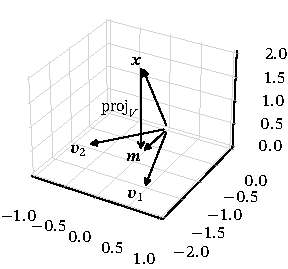
\includegraphics{projection.pdf}
\end{figure}

\subsection{直交補空間}
\begin{figure}[htbp]
  \centering
  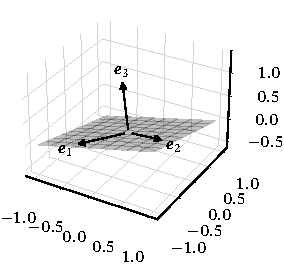
\includegraphics{orthogonal_complement.pdf}
\end{figure}

\subsection{スペクトル定理}

\section{最小二乗問題}

\subsection{最小二乗問題}
\subsection{特異値分解}
\subsection{擬似逆行列}

\section{離散フーリエ変換}

\section{多重解像度解析}

\section{主成分分析}
\begin{figure}[htbp]
  \begin{minipage}{\linewidth/2}
    \centering
    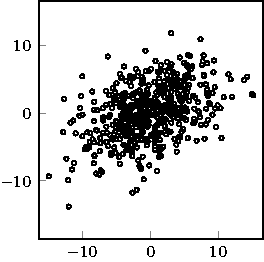
\includegraphics{scatter.pdf}
  \end{minipage}%
  \begin{minipage}{\linewidth/2}
    \centering
    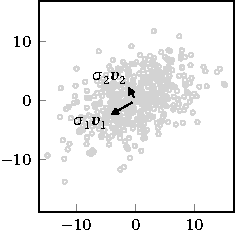
\includegraphics{pca.pdf}
  \end{minipage}
\end{figure}

\begin{subappendices}
\section{低ランク近似}
\end{subappendices}

\section*{演習問題}
\addcontentsline{toc}{section}{演習問題}

\end{document}
